%!TEX root = ../main.tex

\begin{titlepage}

    
\includegraphics[height=2.5cm]{images/cover/logo-dhbw.pdf}
    \IfStrEq{\showCompanyLogo}{true}{
        \hfill
        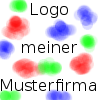
\includegraphics[height=2.5cm]{images/cover/logo-company.png}
    }
    
    \enlargethispage{20mm}
    \begin{center}
        \doublespacing{
            \vspace*{12mm}
            {\LARGE\textbf\documentTitle}
        }\\
        \vspace*{12mm}
        {\large\textbf\documentTypePhrase}\\

        % degre only for bachelor thesis
        \ifDocType{T3300}{
            \vspace*{12mm}
            \degreePhrase\\
            \vspace*{3mm}
            {\textbf\degree}\\
        }

        \IfStrEq{\showLecture}{true}{
            \vspace*{12mm}
            \lecturePhrase\\
            \vspace*{0mm}
            {\textbf\lecture}\\
        }

        \vspace*{12mm}\departmentPhrase\space\department\\
        \vspace*{0mm}\locationUniversityPhrase{} \locationUniversity\\
        \vspace*{12mm}\documentAuthorPhrase\\
        \vspace*{3mm}
        {\large\textbf\documentAuthor}\\
        \vspace*{12mm}\releaseDate\\
        \vfill
        \begin{spacing}{0.8}
            % Eigene Dokumenttypen (z. B. Konzeptarbeit): ohne Dualen Partner und betrieblichen Betreuer
            \ifSpecialDocument{%
                \begin{tabular}{@{}p{0.47\textwidth}p{0.47\textwidth}@{}}
                    \textbf{\documentPeriodPhrase}                     & \documentPeriod               \\
                    \textbf{\matriculationNumberPhrase, \coursePhrase} & \matriculationNumber, \course \\
                    \textbf{Dozent}                                    & \evaluator
                \end{tabular}%
            }{%
                \begin{tabular}{@{}p{0.47\textwidth}p{0.47\textwidth}@{}}
                    \textbf{\documentPeriodPhrase}                     & \documentPeriod                \\
                    \textbf{\matriculationNumberPhrase, \coursePhrase} & \matriculationNumber, \course  \\
                    \textbf{\companyPhrase}                            & \companyName, \companyLocation \\
                    \textbf{\tutorPhrase}                              & \tutor                         \\
                    \textbf{\evaluatorPhrase}                          & \evaluator
                \end{tabular}%
            }
        \end{spacing}
    \end{center}
\end{titlepage}
